\chapter{Block-Graphen}
\section{Blöcke}
\begin{definition}
    Sei $G = (V,E)$. Wir definieren eine Äquivalenzrelation auf $E$ wie folgt:
    $$e \sim f: \Leftrightarrow e = f \text{  oder  } \exists \text{ Kreis durch } e \text{ und } f$$
\end{definition}
\bigskip

Diese Äquivalenzklassen nennen wir auch \textbf{Blöcke}. Eine alternative Definition lautet wiefolgt:

\begin{definition}
    Sei $G = (V,E)$ ein zusammenhängender Graph. Ein \textbf{Block} ist eine maximale Menge von Kanten, so
    dass je zwei dieser Kanten auf einem gemeinsamen Kreis liegen.
\end{definition}
\bigskip

Merke: Ein Block ist ein Subgraph, der 2-zusammenhängend ist.

\begin{lemma}
    Zwei Blöcke schneiden sich - wenn überhaupt - immer in einem Artikulationsknoten.
\end{lemma}
\bigskip

Wir erinnern uns an die Definition von bipartiten Graphen.

\begin{definition}
    Ein Graph ist \textbf{bipartit}, wenn sich die Knotenmenge in zwei disjunkte Mengen
    $A$ und $B$ zerlegen lässt, sodass Kanten von $G$ nur zwischen $A$ und $B$ verlaufen.
    Wir verwenden dafür folgende Notation:
    $$V = A \uplus B$$
\end{definition}
\bigskip


\section{Block-Graphen}
Ein Block-Graph ist nun wiefolgt definitert:

\begin{definition}
    Der Block-Graph von $G$ ist der bipartite Graph $T = (A \uplus B, E_T )$ mit
    \begin{itemize}
        \item $A =$ {Artikulationsknoten von $G$}
        \item $B =$ {Blöcke von $G$}
        \item $\forall a \in A , b \in B: \{a,b\} \in E_T \Leftrightarrow a$ inzident zu einer Kante in $b$
    \end{itemize}
\end{definition}
\bigskip

\begin{figure}[h]
    \centering
    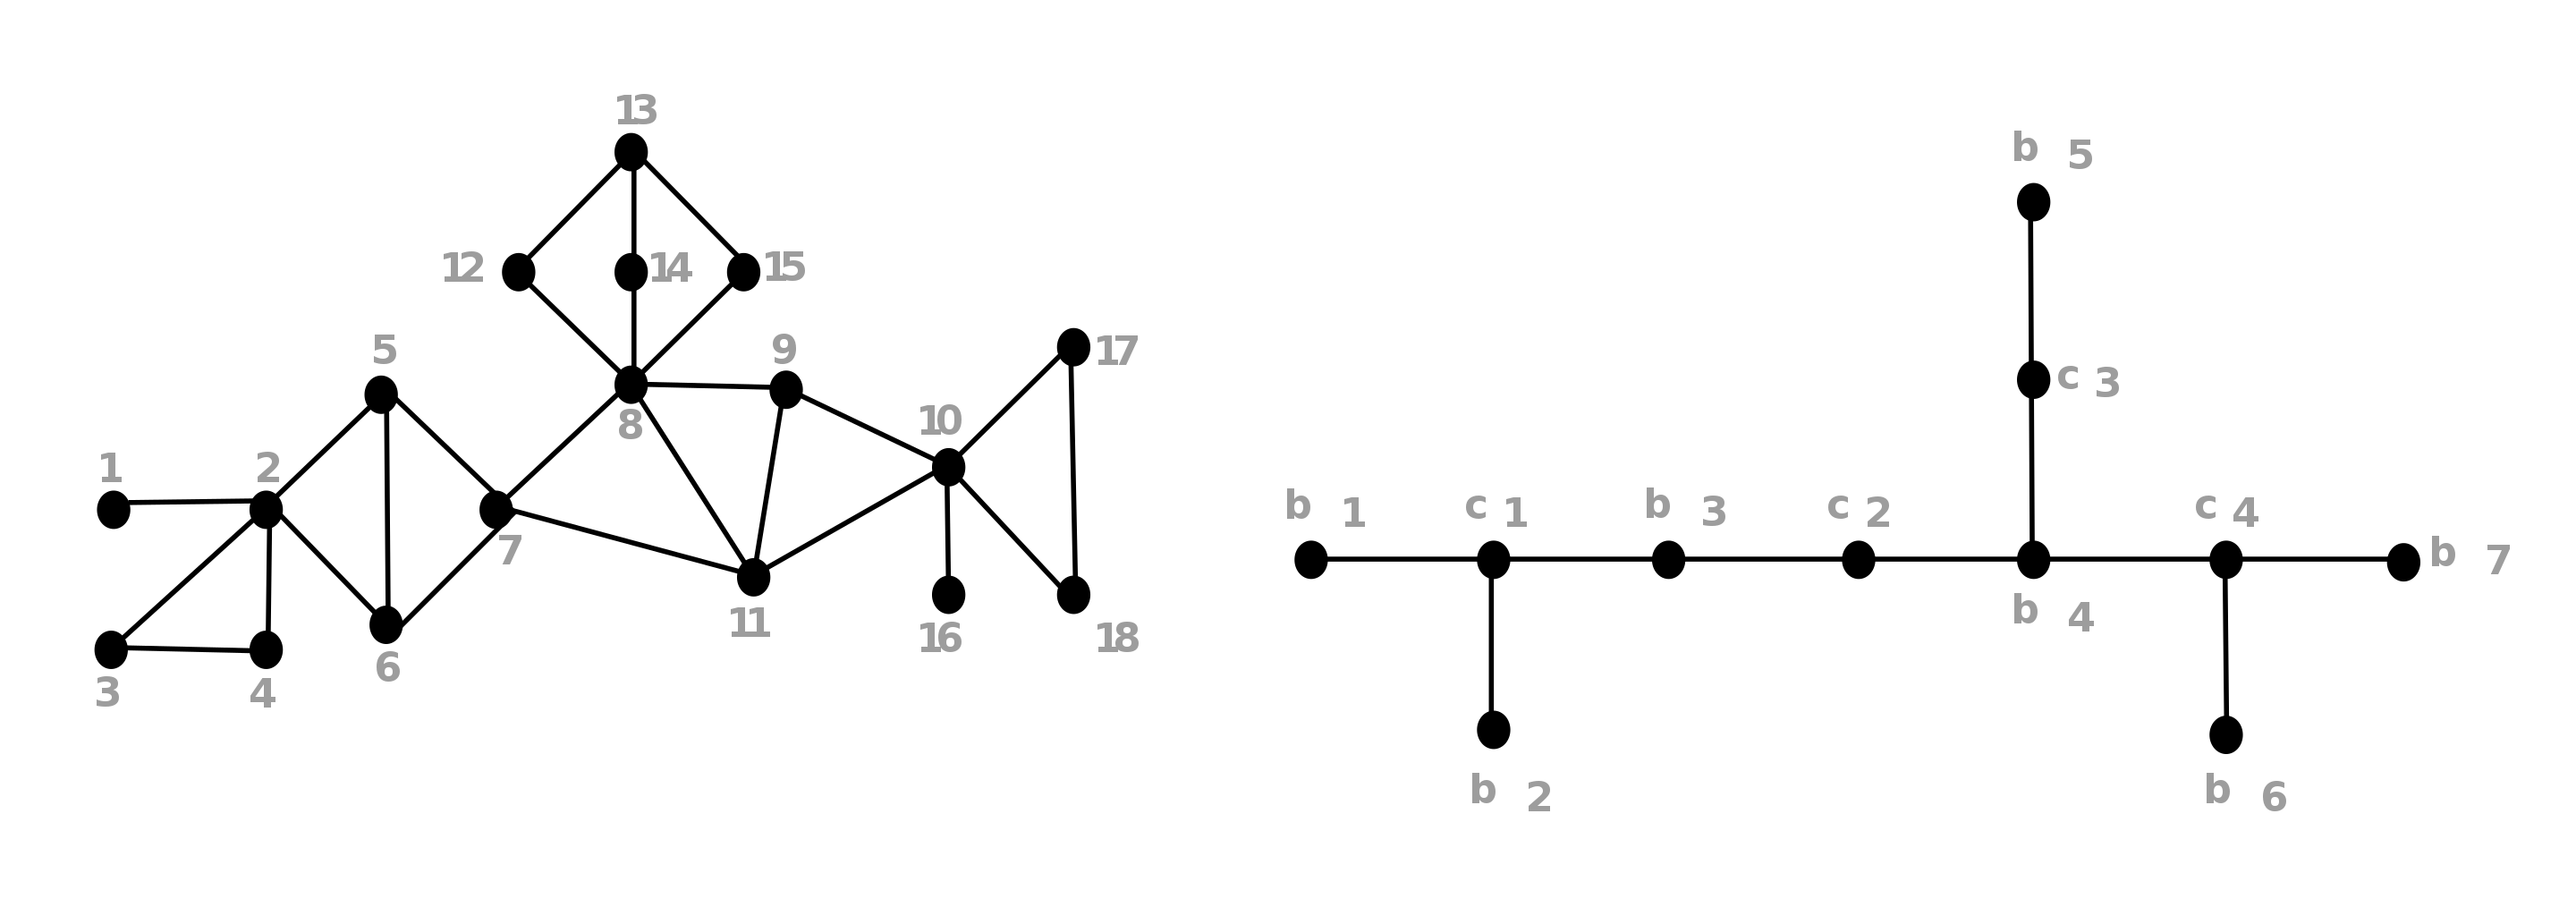
\includegraphics[width=\textwidth]{block_graph.png}
    \caption{Beispiel eines Block-Graphen (links) und der }
\end{figure}